% !Mode:: "TeX:UTF-8"
% -*-coding: utf-8 -*-

% Русский язык дополнительно настраивать не нужно.
% Убедитесь, что ваш редактор поддерживает UTF-8.
\documentclass{math-mech-sci}

% Название и авторы задаются при помощи специальных
% команд \deftitle и \defauthor. Специальные команды
% требуются для генерации корректной метаинформации в
% PDF-файле.

% Блоки в квадратных скобках опциональны, они предназначены
% для сносок на гранты, которыми поддержана работа.

\deftitle
  {О редукции параметров в моделях  сложных  распределений с применением в радиобиологии}

\defauthor%
  {Олейник М. В.}%
  {СПбГУ, Санкт-Петербург}%
  {st087252@student.spbu.ru}
\defauthor
  {Алексеева Н.П.}%
  {СПбГУ, Санкт-Петербург}%
  {nina.alekseeva@spbu.ru}

\begin{document}

	\maketitle
	
	\begin{abstract}
		
	В данной статье рассматривается возможность применения двухпараметрической модели  сложного логарифмически-пуассоновского распределения для описания динамики роста числа аномалий на ядрах клеток рабдомиосаркомы в зависимости от облучения. Приведены вероятности распределения  с применением чисел Стирлинга второго рода и Эйлера. Приведено   обоснование возникновения этих специальных чисел  через ряды по упорядоченным разбиениям.  
	
	\end{abstract}
	
	\section{Введение}
	
%	Распределение случайной величины, которую можно представить в виде случайной суммы независимых одинаково распределенных случайных величин, относится к так называемым сложным распределениям.
%	
%	Несмотря на то что нахождение модели для данных может оказаться достаточно трудоёмким процессом, интерпретация и упрощение оказывается даже более важным этапом исследования. Многопараметрические  модели могут давать хорошее согласование по хи-квадрату при оценке параметров методом максимального правдоподобия ввиду своей гибкости, однако это может говорить о её избыточности.
	
	Для радиобиологических данных числа аномалий в ядрах клеток рабдомиосаркомы у крыс при облучении  разной степени интенсивности в экспериментах in vivo и in vitro ранее была исследована модель реинтрантного бинома с двумя парами неизвестных параметров. В поисках адекватных моделей  с меньшим числом параметров  рассматривались разные варианты, сначала обобщение отрицательного биномиального распределения за счет перехода от пуассоновского распределения числа слагаемых к биномиальному --- биномиально-логарифмического, затем  его антипод --- логарифмически-биномиальное распределение. Предварительная оценка параметров указала на преимущество последнего в предельном случае, соответствующем пуассоновскому распределению случайных компонент. В данной статье изучаются  модели пуассон-логарифмического  (отрицательно-биномиальное) и логарифмически-пуассоновское (ЛПР).  Эти двухпараметрические модели показали удовлетворительное  согласование с эмпирическими данными.
	
	Наиболее адекватной для интерпретации оказалась модель  ЛПР. Соотношение между оценками параметров  логарифмического и пуассоновского распределений свидетельствуют об интенсивном характере  образования аномалий в эксперименте in vivo и экстенсивном в эксперименте in vitro.
	
	\section{Логарифмически-пуассоновское распределение}
	
	Логарифмически-пуассоновское распределение вводится как распределение  случайной суммы независимых случайных величин
	\[
		\zeta_\tau = \xi _1 + \dots + \xi _\tau,
	\]
	где $\xi _i$ имеют распределение Пуассона с параметром $\lambda$,  и производящей функцией $g(t) = e ^{\lambda(t - 1)}$, а $\tau$ --- логарифмическое  с  вероятностями
	\[
		P(\tau = j) = \frac {\alpha q ^j} {j}, \text{где}~ \alpha = -(\ln(1 - q)) ^{-1}, \quad j = 1, 2, \dots 
	\]
	с производящей функцией $f(t) = -\alpha \ln(1 - qt)$.
%
		Согласно \cite{bib:feller1952}, производящая функция случайной величины $\zeta$ имеет вид суперпозиции производящих функций  логарифмического и пуассоновского распределений,
			\begin{equation}\label{lpr:pfm}
			h (t) = -\alpha \ln (1 - q e ^{\lambda (t - 1)})\,.
		\end{equation}
%		
%	
%	Получить его также можно из сведения логарифмически-биномиального распределения к распределению с меньшим количеством параметров. Для этого устремим параметр $n$ к бесконечности, а $p$ к нулю так, чтобы $n \cdot p = \lambda$. По теореме Пуассона, таким образом, из биномиального распределения получается распределение Пуассона. 
%	
%	Очевидным преимуществом данного распределения является вещественность всех его параметров, а также, в принципе, их количество: два против трёх. Однако было утеряно свойство переменности знака логарифма рассеяния.
%
%	%\section{Вероятности}
%	

	
	\textbf{Теорема 1.}
%		Обозначим $\alpha = -1 / \ln(1 - q)$.
%		
Обозначим через $S(k, j)$ числа Стирлинга второго рода~\cite{bib:knuth1998}, имеющие следующую рекуррентную формулу:
\[
S(k, j) = S(k - 1, j - 1) + j \cdot S(k - 1, j), \quad 0 < j \leqslant k,
\]
$
S(0, 0) = 1, S(k, 0) = 0~ \text{при}~ k > 0, S(k, j) = 0~ \text{при}~ j > k.
$
		Пусть  $Q(\lambda,q)=\frac {q e ^{-\lambda}} {1 - q e ^{-\lambda}}$, где  $\lambda > 0$ и $q \in (0, 1)$.   Тогда вероятности логарифмически-пуассоновского распределения с параметрами $\lambda$,  $q $  и с  производящей функцией (\ref{lpr:pfm}) имеют вид:
		\begin{equation}\label{lpr:prob1}
			P(\zeta _\tau = k) = \frac \alpha {k !} \lambda ^k \sum \limits _{j = 1} ^{k} (j - 1)! S(k, j) Q(\lambda,q)^j \mbox{  при } k = 1, 2 \dots.,
		\end{equation}
	\[
	P(\zeta_\tau = 0) = -\alpha \ln\left(1 - q e ^{-\lambda}\right)\,.
	\]
			Вероятности (\ref{lpr:prob1}) получены через формулу для производящих функций:
	$ 
	P(S _\tau = k) = \frac {1} {k!} h ^{(k)} (0), \quad k = 0, 1, 2, \dots, 
$
	а доказательство теоремы осуществлено по методу математической индукции.
%	
%	Приведём небольшую часть таблицы чисел Стирлинга:
%	\begin{center}
%		\[
%		\begin{array}{c|cccccccc}
%			k\textbackslash j & 0 & 1 & 2 & 3 & 4 & 5 & 6\\ \hline
%			0 & 1 &   &  &  & &  &\\
%			1 & 0 & 1 &  &  & &  &\\
%			2 & 0 & 1 & 1 &  & &  &\\
%			3 & 0 & 1 & 3 & 1 &  & &\\
%			4 & 0 & 1 & 7 &  6 & 1 & & \\
%			5 & 0 & 1 & 15 & 25 &10 &1 & \\
%			6 & 0 & 1 & 31 & 90 & 65 & 15 & 1
%		\end{array}
%		\]
%	\end{center}
%	
Для чисел Стирлинга второго рода  известна явная формула
$
	S(k, j) = \frac {1} {j!} \sum \limits _{i = 0} ^j (-1) ^{j + i} C _{j} ^{i} i ^k, 
$
	поэтому не видно  никаких ограничений для использования (\ref{lpr:prob1}). Однако вероятности 
	(\ref{lpr:prob1})  можно получить при помощи  специальных чисел  другого вида. Также методом математической индукции
		доказано следующее утверждение. 

	\textbf{Теорема 2.}
	Обозначим через  $E(k, j)$  числа Эйлера первого рода~\cite{bib:knuth1998} для которых справедлива  рекуррентная формула:
	\[
	E(k, j) = (j + 1) \cdot E(k - 1, j) + (k - j) \cdot E(k - 1, j - 1), 0 < j < k - 1,
	\]
	\[
	E(k, 0) = 1~ \text{при}~ k \geqslant 0, E(k, j) = 0~ \text{при}~ j \geqslant k > 0.
	\]
%
		Вероятности логарифмически-пуассоновского распределения для $k>0$ могут быть выражены следующим образом:
	%
			\begin{equation}\label{lpr:prob2}
				P( \zeta _\tau = k) = \frac \alpha {k !} \frac {\lambda ^k q e ^{-\lambda}} {\left(1 - q e ^{-\lambda}\right) ^k} \sum \limits _{j = 0} ^{k - 2} E(k - 1, j) \left(q e ^{-\lambda}\right) ^j\,.
			\end{equation}
			
	

	
	Числа Эйлера (табл.\ref{tab1}) представляют собой количество перестановок порядка $k$ с $j$ подъёмами, то есть в перестановке $\pi = (\pi _1, \dots, \pi _k)$ всего $j$ индексов $i$ таких, что $\pi _i < \pi _{i + 1}$. 
		
		
		\begin{table}[ht]\centering\begin{tabular}{c|cccccc}
	
			k $\backslash$ j & 0 & 1 & 2 & 3 & 4 & 5\\ \hline
			0 & 1 &  &  &  &  & \\
			1 & 1 &  &  &  &  & \\
			2 & 1 & 1 &  &  &  & \\
			3 & 1 & 4 & 1 &  &  & \\
			4 & 1 & 11 & 11 & 1 &  & \\
			5 & 1 & 26 & 66 & 26 & 1 & \\
			6 & 1 & 57 & 302 & 302 &57 &1 \\
		\end{tabular}
	\caption{Числа Эйлера.}
	\label{tab1}
	\end{table}
	Эти числа, явный вид которых 
$
	E(k, j) = \sum \limits ^j _{i = 0} C ^i _{k + 1} (-1) ^i (j + 1 - i) ^k,
$
	возникают также в функциональном  ряде
	\[
		\sum \limits ^\infty _{i = 1} i ^k x ^i = \frac {x} {(1 - x) ^{k + 1}} \sum \limits ^{k - 1} _{j = 0} E(k, j) x ^j, 
	\]
	который  в нашем случае возникает 
%	Убедимся в справедливости этого утверждения. Используем 
при использовании формулы полной вероятности
%, чтобы найти вероятность случайной суммы случайных величин:
	\[
	\begin{aligned}
		P(\zeta_\tau = k) =& \sum \limits ^{\infty} _{j = 1} P(\left.\zeta_\tau = k\right| \tau = j) \cdot P(\tau = j) =\\
		=& \sum \limits ^{\infty} _{j = 1} - \frac 1 {\ln(1 - q)} \frac {q ^j} j \frac {(j \lambda) ^k} {k !} e ^{-j \lambda} = \frac \alpha {k !} \lambda ^k \sum \limits ^{\infty} _{j = 1} j ^{k - 1} \left(q e ^{-\lambda}\right) ^j \,.
%		=\\
%		=& \frac \alpha {k !} \frac {\lambda ^k q e ^{-\lambda}} {\left(1 - q e ^{-\lambda}\right) ^k} \sum \limits ^{k - 2} _{j = 0} E(k - 1, j) \left(q e ^{-\lambda}\right) ^j.
	\end{aligned}
	\]
	
%	
%	Компьютерное вычисление вероятностей показало эквивалентность этих трёх формул с погрешностью на уровне машинного нуля.
	
	\section{Оценка параметров и пример из  радиобиологии }
	
	\begin{figure}[!h]
		\centering
		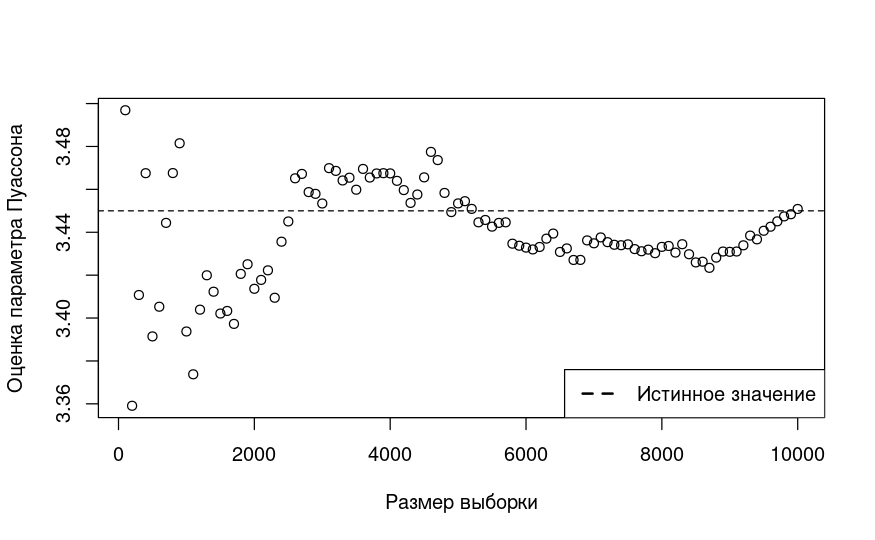
\includegraphics[width = 0.5\textwidth]{logpoislambda}
		\caption{Сходимость оценки параметра $\lambda$ к истинному значению для логарифмически-пуассоновского распределения.}
		\label{img:logpoislambda}
	\end{figure}
	
	\begin{figure}[!h]
		\centering
		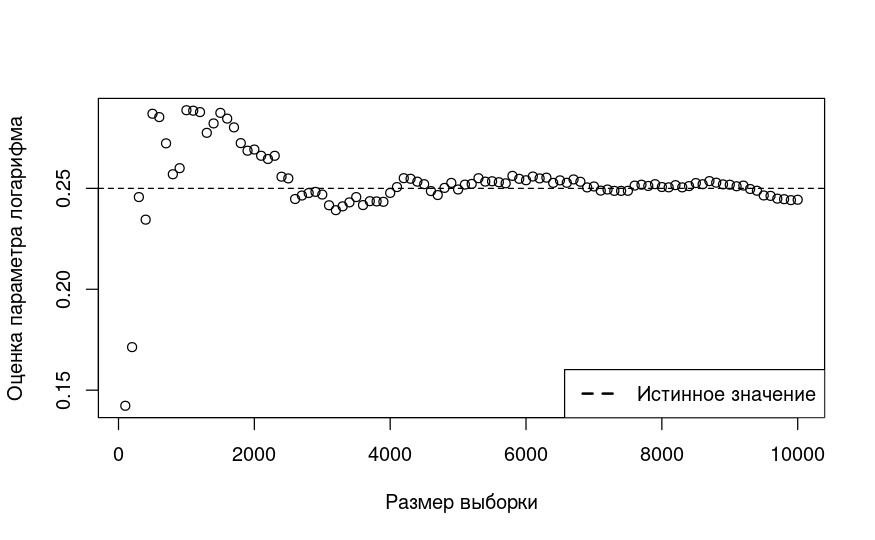
\includegraphics[width = 0.5\textwidth]{logpoisq}
		\caption{Сходимость оценки параметра $q$ к истинному значению для логарифмически-пуассоновского распределения.}
		\label{img:logpoisq}
	\end{figure}
	
	Оценка параметров $\lambda$ и $q$ проводилась методом максимального правдоподобия численно на компьютере с использованием функции \verb|optim| на языке \verb|R|.
	%
	Моделируя выборку из $n$ индивидов для известных параметров можно проверить состоятельность такой оценки (рис.~\ref{img:logpoislambda}, \ref{img:logpoisq}).
	
	
	
	\begin{table}[!ht]
		\centering
		\footnotesize
		\begin{minipage}{0.4\textwidth}
			\centering
			\caption*{In vivo}
			\begin{tabular}{rrrr}
				\hline
				Гр & $\lambda$ & $q$ & \textbf{p-v} \\ 
				\hline
				0 & 0.38 & 5.9e-7 & \textbf{0.13} \\ 
				5 & 0.67 & 3.3e-7 & \textbf{0.81} \\ 
				10 & 0.83 & 6.7e-7 & \textbf{0.21} \\ 
				15 & 1.15 & 5.3e-7 & \textbf{0.01} \\ 
				20 & 1.71 & 1e-5 & \textbf{0.03} \\ 
				25 & 1.04 & 0.07 & \textbf{0.55} \\ 
				30 & 1.48 & 0.33 & \textbf{0.33} \\ 
				35 & 1.75 & 0.19 & \textbf{0.11} \\ 
				40 & 2.05 & 0.22 & \textbf{0.16} \\
				45 & 2.36 & 0.18 & \textbf{0.08} \\ 
				\hline
			\end{tabular}
			\label{tab:logpoisvivo}
		\end{minipage}
		\begin{minipage}{0.4\textwidth}
			\centering
			\caption*{In vitro}
			\begin{tabular}{rrrr}
				\hline
				Гр & $\lambda$ & $q$ & \textbf{p-v} \\ 
				\hline
				0 & 0.39 & 3.7e-6 & \textbf{0.59} \\ 
				5 & 0.14 & 0.80 & \textbf{0.73} \\ 
				10 & 0.59 & 1.1e-7 & \textbf{0.03} \\ 
				15 & 0.41 & 0.76 & \textbf{0.36} \\ 
				20 & 0.37 & 0.56 & \textbf{0.45} \\ 
				25 & 0.88 & 0.37 & \textbf{0.22} \\ 
				30 & 0.78 & 0.53 & \textbf{0.26} \\ 
				35 & 1.10 & 0.43 & \textbf{0.43} \\ 
				40 & 1.46 & 0.29 & \textbf{0.38} \\ 
				\hline
			\end{tabular}
			\label{tab:logpoisvitro}
		\end{minipage}
		\caption{Оценки параметров и значимости критерия хи-квадрат по данным in vivo и in vitro для логарифмически-пуассоновского распределения.}
		\label{tab:logpois}
	\end{table}
	
	В таблице~\ref{tab:logpois} представлены оценки параметров для радиобиологических данных из статьи~\cite{bib:alexeeva2008}, а также показано согласие с эмпирическим распределением.
	%
	При уровне значимости $\alpha = 0.05$ получаем согласие для $16 / 19 \cdot 100 \% = 84 \%$ случаев. 
	
	%\subsection{Интерпретация}
	
	\begin{figure}[!h]
		\centering
		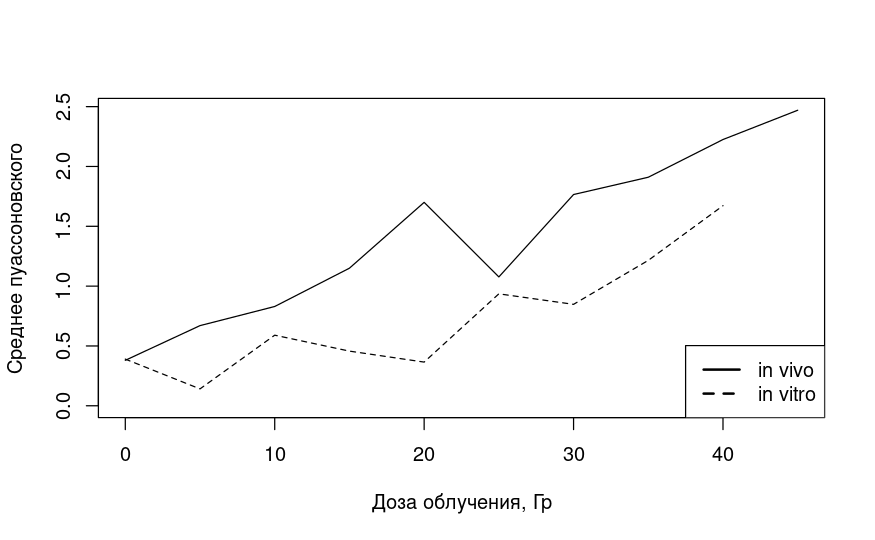
\includegraphics[width = 0.6\textwidth]{logpoismeanpois}
		\caption{Оценка параметра $\lambda$  в зависимости от дозы облучения}
		\label{img:logpoismeanpois}
	\end{figure}
	
	\begin{figure}[!h]
		\centering
		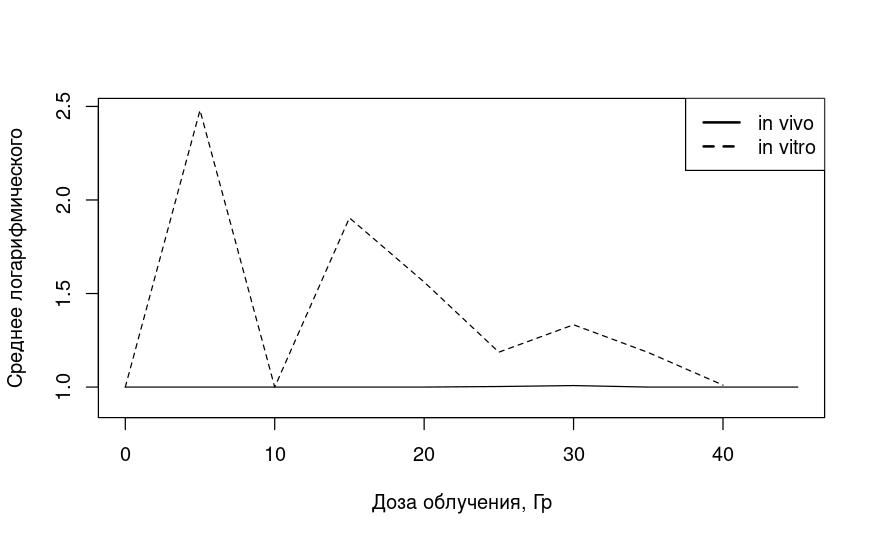
\includegraphics[width = 0.6\textwidth]{logpoismeanlog}
		\caption{Среднее  лог. распределения  в зависимости от дозы облучения}
		\label{img:logpoismeanlog}
	\end{figure}

	Наблюдаемое количество аномалий определяется в целом двумя факторами: их исходной распространенностью и интенсивностью их образования в процессе митоза. За увеличение исходной  распространенности отвечает параметр $q$ логарифмического распределения, а за интенсивность образования аномалий в процессе митоза параметр $\lambda$  пуассоновского распределения. Поскольку распределения  суммы и самих случайных величин однопараметрические, при интерпретации  параметров можно опираться на их средние значения.
	
	Динамика оценок параметра $\lambda$,  соответственно средних значений, свидетельствует о положительной линейной зависимости их от дозы облучения, что очевидно, и о значимо меньших значениях в эксперименте in vitro (рис.~\ref{img:logpoismeanpois}), так как выжившие клетки обладают большим иммунитетом. 
	
	Что касается исходной распространенности аномалий, то, согласно динамике оценок параметра $q$  в зависимости от дозы облучения (рис.~\ref{img:logpoismeanlog}), зависимости от дозы облучения нет, а в эксперименте in vivo базовая распространенность практически не выражена и существенно меньше, чем в эксперименте in vitro. Это объясняется тем, что от дозы облучения зависит только количество выживших клеток, а не распространенность их аномалий, которая, судя по графику,   очень вариабельна, но существенно выше базовой распространенности до начала эксперимента.
	
	\section{Обобщение на случай произвольных распределений}
	
Рассмотрим модель сложного распределения  $\zeta_\tau=\xi_1+\ldots+\xi_\tau$, в котором случайное число слагаемых $\tau$ распределено по $(P_0,P_1,P_2,\ldots)$,  а независимые компоненты по $(p_0, p_1,p_2,\ldots)$. 
Вероятности сложного закона распределения можно выразить через  конечную суммы
	%
\[
	P\{\zeta_\tau=n\}=\frac 1{n!}\sum\limits_{k=1}^n \Theta_k G_n^k\,,~~~
	\mbox{где}~~
	\Theta_k=\sum\limits_{i=k}^\infty P_iC_i^{i-k} p_0^{i-k}\,,
	%
	\]
	\[
	G_n^k=n!\sum\limits_{\sum_i^k n_i=n}\prod\limits_{i=1}^kp_{n_k}
	\]
	%
	 и $n=(n_1,\ldots,n_k), n_i>0,$ 
упорядоченные разбиения  натурального числа $n$.  
%Можно показать, что число таких разбиений равно $C_{n-1}^{k-1}$ --- число сочетаний расстановки разделителей, чтобы получить $k$  агрегаций. 
%
%Алгоритм для вычисления $G_n^k$ достаточно прост.  Например, нужно вычислить $G_5^3$. Для этого перебираем $C_4^2=6$ сочетаний
%12, 13, 14, 23, 24, 34 
%и с их помощью разбиваем последовательность $\Omega_5=(1,2,3,4,5)$, расставляя вместо  запятых разделитель, например, для 1-й и 2-й запятой получим 1-2-345, для 1-й и 3-й 1-23-45 и так далее. 
%
%$$
%\begin{array}{c|c|c|c|c}
%	\hline
%	\mbox{зап.1} & \mbox{зап.2} & \mbox{разбиение} & \mbox{успехи} & \mbox{вер-ть}\\
%	\hline
%	1 & 2 &  1-2-345 & *-*-*** & p_1^2p_3\\
%	1 & 3 &  1-23-45 & *-**-** & p_1p_2^2\\
%	1 & 4 &  1-234-5 & *-***-* & p_1^2p_3\\
%	2 & 3 &  12-3-45 & **-*-** & p_1p_2^2\\
%	2 & 4 &  12-34-5 & **-**-* & p_1p_2^2\\
%	3 & 4 &  123-4-5 & ***-*-* & p_1^2p_3\\
%\end{array}
%$$
Сравнивая  выражения $G_n^k$ в случае  логарифмических и  пуассоновских независимых величин, приходим  к двум видам суммирования над упорядоченными разбиениями:
%
%Если представлять  $\tau$ как случайное число веток, на которых появляются случайное число листьев, то компонента  $G_n^k$ будет  означать вероятность появления $n$ листьев на $k$ живых ветках, а 
%$Q_k(1-p_0)^k$ вероятность того, что с листьями  окажутся $k$ веток. 
%	
%	
%
$$
	u_n^k=\sum\limits_{ \sum_i^k n_i=n,n_i>0 } \frac{n!}{ n_1\ldots n_k},~~~~~~
		v_n^k=\sum\limits_{ \sum_i^kn_i=n,n_i>0} \frac{n!}{n_1!\ldots n_k!}
$$
	с рекуррентными соотношениями 
	$$
	u_n^k=ku_{n-1}^{k-1} +(n-1)u_{n-1}^k\,,~~~~~v_n^k=k(v_{n-1}^{k-1} +v_{n-1}^k)\,,
	$$
	которые приводят к 
существенным частным случаям в виде чисел Стирлинга первого и второго рода
$
s(n,k)=\frac 1{k!}u_n^k $  и  $S(n,k)=\frac 1{k!}v_n^k\,.
$
В случае пуассоновского распределения независимых компонент  сумма по упорядоченным разбиениям имеет тип  $v_n^k$, а в случае логарифмического  тип $u_n^k$. 

%	 Закон распределения $\tau$  отражается на выражениях для  $\Theta_k$.  
При логарифмическом  распределении   (\ref{lpr:prob1}) числа компонент $\tau$  имеем  $\Theta_k=\frac\alpha k\left( \frac q{1-qp_0}\right)^k$ ,  а при пуассоновском 
 $\Theta_k=\frac{\lambda^k}{k!}e^{-\lambda+\lambda p_0}$. Отличие  в константах  $\frac 1 k$ или $\frac 1 {k!}$ приводит к разному виду коэффициентов. Например, пуассоновское $\tau$ с внутренним логарифмическим дает сочетание $\frac 1{k!}u_n^k$, приводящее напрямую к степенному ряду с коэффициентами в виде чисел Стирлинга первого рода,  соответственно к  убывающему факториалу и к вероятностям отрицательного  биномиального  распределения. Реинтрантный пуассон приводит к вероятностям с весами в виде чисел Стирлинга второго рода, реинтрантный логарифм или логарифм-пуассон дадут соответственно  взвешенные числа Стирлинга первого и второго рода вида $(k-1)!s(n,k)$  и $(k-1)!S(n,k)$.  

	\section{Заключение}
	
	Конечные суммы над упорядоченными разбиениями, связанные с числами Стирлинга, позволяют систематизировать разные виды сложных распределений и тем самым  ускорить процесс выбора наиболее адекватной модели. 
	
	
	\begin{thebibliography}{8}
	
	\bibitem{bib:alexeeva2008} Динамика роста числа ядерных аномалий
	рабдомиосаркомы RA-23 при увеличении дозы острого редкоионизирующего облучения. Исследование на основе модели реинтрантно-биномиального распределения~/ Алексеева~Н.~П., Алексеев~А.~О., Вахтин~Ю.~Б., Кравцов~В.~Ю., Кузоватов~С.~Н. и Скорикова~Т.~И.~// Цитология. 2008. --- С.~528--534.
	
	\bibitem{bib:feller1952} Феллер~В. Введение в теорию вероятностей и её приложения. В 2 т.
	\newblock Москва~: Мир, 1952.
	\newblock Т.~1.
	
	\bibitem{bib:knuth1998} Грэхем~Р., Кнут~Д., Паташник~О. Конкретная
	математика. Основание информатики.
	\newblock Москва~: Мир, 1998.
	\newblock ISBN:~\href{http://isbndb.com/search-all.html?kw=5-03-001793-3}{5-03-001793-3}.
	
	\end{thebibliography}

\end{document}
